\documentclass[journal,12pt,twocolumn]{IEEEtran}
\usepackage{hyperref}
\usepackage{graphicx}
\usepackage{amsmath}
\title{Assignment 2}
\author{JARPULA BHANU PRASAD - AI21BTECH11015}
\date{Aptil 2021}
\begin{document}
\maketitle
\noindent \Large\underline{Download codes from}:
\fbox{\begin{minipage}[t]{0.95\columnwidth}
\large Download python code from - \href{https://github.com/jarpula-Bhanu/Assignment-2/blob/main/codes/function.py}{Python}\\Download latex code from - \href{https://github.com/jarpula-Bhanu/Assignment-2/blob/main/Assignment2.tex}{Latex}
\end{minipage}}

\section{\Large\underline{Problem-ICSE-2019-12 Q)4-b}}
\large\noindent Q) If $f$ : A $\rightarrow$ A and A = $R$ - \{$\frac{8}{5}$\} , show that the function $f(x)$ = $\frac{8x+3}{5x-8}$ is one-one onto. Hence, find $f^{-1}$. 
\section{\large\underline{Solution}}
\fbox{\begin{minipage}[t]{0.95\columnwidth}
\noindent \underline{Definition}: Let $f$ : $X$ $\rightarrow$ $Y$ be a function, we say $f$ is one-one or injective,\\if and only if $\forall$ $x_1$ , $x_2$ $\in$ $X$.\\ if $f(x_1)$ = $f(x_2)$ then $x_1$ = $x_2$.
\end{minipage}}
\vspace{5mm}

\noindent Suppose that $x_1$ and $x_2$ are arbitrary integers and $f(x_1)$ = $f(x_2)$, we need to show that $x_1$ = $x_2$. Since $f(x_1)$ = $f(x_2)$.\\
\begin{align*}
f(x_1)=\frac{8x_1+3}{5x_1-8} \hspace{5mm} and \hspace{5mm} f(x_2)=\frac{8x_2+3}{5x_2-8}
\end{align*}\\
\noindent Now, equating $f(x_1)$ = $f(x_2)$ since from the defination.
\begin{align} \label{1}
\implies \frac{8x_1+3}{5x_1-8} = \frac{8x_2+3}{5x_2-8}
\end{align}
On cross multiplying and simplifying the eqn\eqref{1}, we get,
\begin{align} \label{2}
\implies 49(x_1 - x_2) = 0.
\end{align}
From the eqn\eqref{2} we can say that,\\ the equation satisfies only when $x_1 - x_2$= 0. Which implies,
\begin{align*}
\Large\framebox[1.2\width]{$x_1$ = $x_2$}
\end{align*}
Hence, the given function $f(x)$ is one-one.

\vspace{5mm}
\fbox{\begin{minipage}[t]{0.95\columnwidth}
\noindent \underline{Definition}: $f$ is called onto if $f(X) = Y$.\\
i.e., Range of the function $f(x)$ is equal to co-domain.
\end{minipage}}
\vspace{5mm}

\noindent Let,
\begin{align} \label{3}
y = f(x) = \frac{8x+3}{5x-8}
\end{align}

On solving the eqn\eqref{3},\\ we get,
\begin{align} \label{4}
\LARGE\framebox[1.2\width]{$x$ = $\frac{8y+3}{5y-8}$}
\end{align}

Where $y$ is element of co-domain.\\ Now eqn\eqref{4} is defined $\forall$ $y$ $\in$ $R$ - \{$\frac{8}{5}$\}.\\ i.e.$y \in$ A.
\vspace{5mm}

\noindent From eqn\eqref{4} we can say $x$ = $\frac{8y+3}{5y-8}$ is continuous  $\forall$ $y$ $\in$ $R$ - \{$\frac{8}{5}$\}.\\
Now for continuous function there are no discontinuous points in domain \\
Hence, we can say for every element in domain there must exist an image. \\ Which impels that given function eqn\eqref{4} (continuous function) is onto. Since co-domain = range (from definition).\\
\noindent now, from eqn\eqref{4} substitute the value of $x$.
\begin{align}
&\implies f(x) = f\bigg\{\frac{8y+3}{5y-8}\bigg\} \\
&\implies f(x) = \frac{8(\frac{8y+3}{5y-8})+3}{5(\frac{8y+3}{5y-8})-8} \\
&\implies f(x) = \frac{8(8y+3)+3(5y-8)}{5(8y+3)-8(5y-8)}\\
&\implies f(x)=\frac{79y}{79} \\
&\implies f(x) = y \label{9}
\end{align}

\noindent Hence, from eqn\eqref{9} we can say, given function $f(x)$ is onto.
\vspace{5mm}

\begin{figure}[h] 
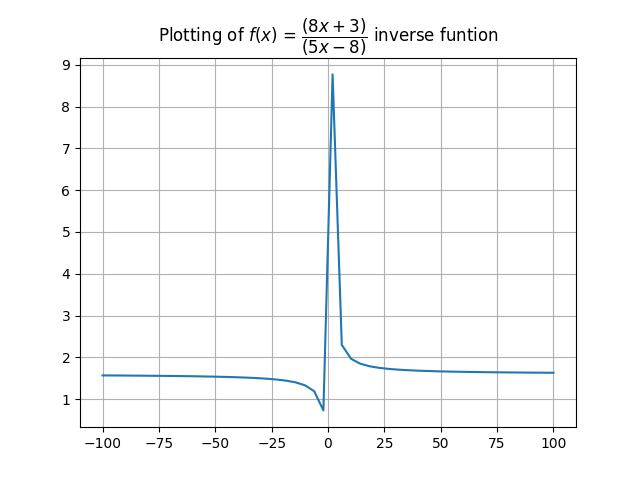
\includegraphics[width=\columnwidth] 
{plotting}
\caption{graph}
\label{fig:a}
\end{figure}

\noindent From the graph \ref{fig:a} we observe that,\\ since the graph is continuous hence it is onto
\noindent
\fbox{\begin{minipage}[t]{0.95\columnwidth}
\noindent\small \underline{NOTE}: The above shown graph is graph of inverse function. In general for inverse function that is not one-one may have multiple images.
\end{minipage}}
\vspace{5mm}

\fbox{\begin{minipage}[t]{0.95\columnwidth}
\noindent \underline{Definition}: $f$: $X$ $\rightarrow$ $Y$ is bijective function i.e., both one-one and onto then there exit a unique function called inverse function and is denoted by $f^{-1}$, such that,
\begin{align*}
f^{-1}(y)=x \iff f(x) = y
\end{align*}
\end{minipage}}
\vspace{5mm}

\noindent Now, from defination $f^{-1}(y)$ = $x$. From eqn\eqref{4} we get the value of $x$ 

\begin{align*}
f^{-1}(y) = \frac{8y+3}{5y-8}
\end{align*}

i.e., the inverse of function $f(x)$ is,
\begin{align*}
\LARGE\framebox[1.2\width]{$f^{-1}(x)$ = $\frac{8x+3}{5x-8}$}
\end{align*}

\end{document}